\iffalse
Possiamo quindi confrontare PICAT con Python. Sono stati entrambi progettati per essere linguaggi di scripting, dinamicamente tipati e permettono side effects. Una delle prime differenze è che anche se previsti PICAT scoraggia l'utilizzo di quest'ultimi mentre in Python ci sono anche funzioni built-in che fanno side effects. Ci sono poi altre differenze tra questi due linguaggi: Python è object oriented a differenza di PICAT che al massimo prevede le strutture, è differente la gestione di liste e array ed inoltre quando un programma PICAT viene compilato, cicli e list comprehension sono trasformati in chiamate tail recoursive in modo da rendere il programma più efficiente, cosa che invece Python non fa
\fi

\begin{frame}{PICAT vs Python}

	\begin{columns}

		\begin{column}{1\textwidth}

			Analogie
			\begin{itemize}
				\item Entrambi pensati come linguaggi di scripting
				\item Dinamicamente tipati
				\item Side effects
			\end{itemize}

			Differenze
			\begin{itemize}
				\item In PICAT l'uso dei side effects è scoraggiato
				\item Python è object oriented a differenza di PICAT
				\item In Python ci sono solo array dinamici mentre in PICAT abbiamo liste e array (non dinamici)
				\item In Python non è supportata l'ottimizzazione con tail recursion
			\end{itemize}

		\end{column}

		\begin{column}{0.1\textwidth}
			\begin{figure}
				\vspace*{-5cm}
				\hspace*{-2cm}
				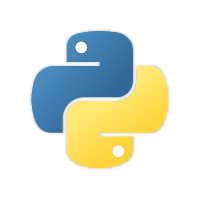
\includegraphics[scale=0.5]{res/pythonLogo}
			\end{figure}
		\end{column}

	\end{columns}


\end{frame}